\chapter{Projeto do sistema}\label{cap:projeto}

O sistema proposto será composto por dois módulos.
O primeiro corresponde à etapa de captura de fotos, detecção facial e upload das faces a serem processadas pelo segundo módulo, que, por sua vez, tenta verificar se a mesma face já foi analisada no passado e extrai características como idade, emoções e gênero.

\section{Módulo 1}\label{sec:modulo1}

O módulo 1 é o foco deste trabalho. Sua principal função é capturar as fotos a serem analisadas no segundo módulo.
Para minimizar o volume de dados trafegados pela rede e concentrar os esforços dos algoritmos de análise apenas nas áreas de interesse, o primeiro módulo não pode enviar todas as imagens capturadas, sendo necessário um pré-processamento que ignore as fotos que não contenham faces e também remova o fundo das fotos que contenham faces.

\subsection{Raspberry Pi}

Câmeras comuns não possuem poder computacional para realizar o pré-processamento desejado e computadores tradicionais são caros, grandes e muito pesados para esse propósito.

O meio termo ideal são os computadores de baixo custo em placa única, que podem ser posicionados de forma discreta e, apesar de limitados, são capazes de executar sistemas operacionais como o Linux ARM.

\begin{figure}[htbp]
    \centering
    \caption{Raspberry Pis com câmera}
    \label{fig:raspberry}
    \begin{subfigure}[t]{0.49\textwidth}
    \centering
    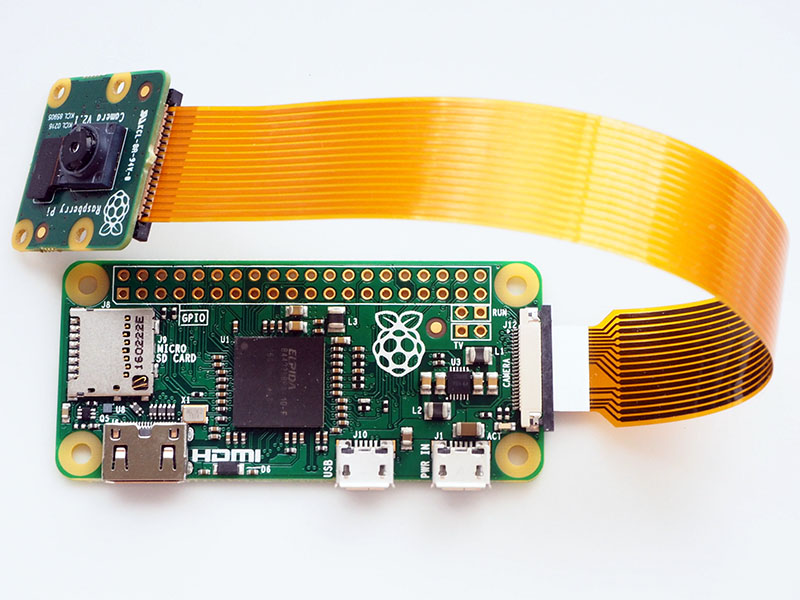
\includegraphics[width=0.95\linewidth]{imagens/raspberry_zero.jpg}
    \caption{Raspberry Pi Zero. Fonte: \cite{upton2016zero}} \label{fig:raspberry:a}
    \end{subfigure}
    \begin{subfigure}[t]{0.49\textwidth}
    \centering
    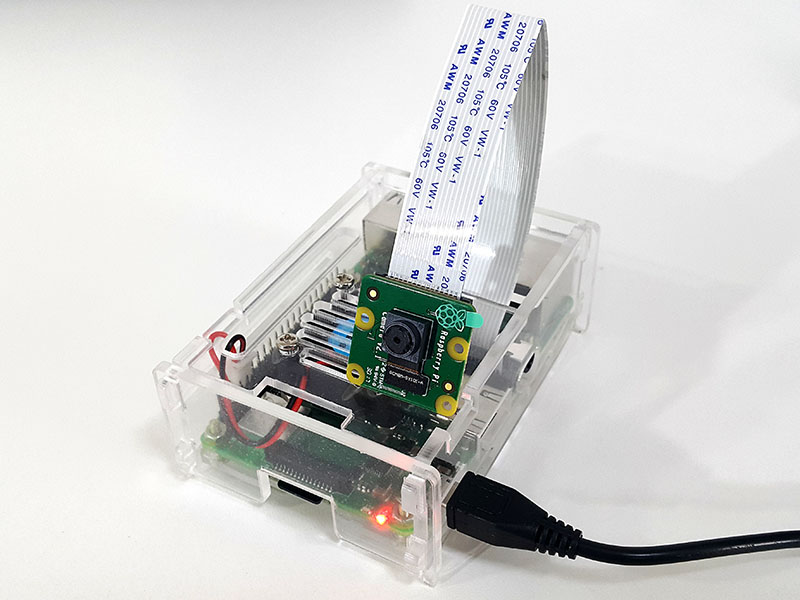
\includegraphics[width=0.95\linewidth]{imagens/raspberry.jpg}
    \caption{Raspberry Pi 3 modelo B+ em um case de acrílico} \label{fig:raspberry:b}
    \end{subfigure}
\end{figure}

O computador escolhido para este projeto foi o Raspberry Pi nos modelos Raspberry Pi Zero (\autoref{fig:raspberry:a}) e Raspberry Pi 3 B+ (\autoref{fig:raspberry:b}) devido ao seu baixo custo, alta disponibilidade e por possuir interface para câmera (CSI). O projeto completo custou menos de R\$ 500,00.

O Raspberry Pi Zero possui um processador ARM single-core de 1 GHz e 512 MB de memória SDRAM, enquanto que o Raspberry Pi 3 modelo B+ possui um processador quad-core 64-bit de 1,4 GHz e 1 GB de memória SDRAM. O Raspberry Pi Zero não possui WiFi e Ethernet como o modelo 3 B+, porém é possível utilizar adaptadores USB para conexão de rede.

O sistema operacional escolhido para ser instalado no Raspberry Pi foi o Raspbian Stretch Lite, uma distribuição de Linux baseada no Debian otimizada especificamente para o Raspberry Pi.

\subsection{Detecção facial}

O programa para selecionar apenas as regiões com faces deve utilizar um algoritmo eficiente de detecção facial capaz de ser executado a pelo menos um quadro por segundo no hardware e sistema operacional escolhidos.

O algoritmo de detecção facial selecionado para o primeiro módulo foi o Viola-Jones, pois, como estudado em capítulos anteriores, ele é eficiente o suficiente para ser executado em tempo real e está implementado na biblioteca multiplataforma OpenCV.

O \autoref{cod:detector_opencv_picamera} apresenta a implementação do sistema de detecção facial utilizando a câmera do Raspberry Pi.

As faces extraídas pelo detector facial, podem ser salvas no cartão de memória para serem acessadas posteriormente ou enviadas pela rede para serem processadas imediatamente.

\section{Módulo 2}\label{sec:modulo2}

O segundo módulo é o responsável por extrair informações das faces enviadas pelo primeiro módulo. Por limitação de armazenamento e processamento, foi decidido que esse módulo não será executado a partir do Raspberry Pi, mas sim em um servidor local ou na nuvem.

Além de reconhecer se uma face já foi analisada no passado, também é desejável estimar informações como idade, sentimento e gênero. Modificações do Eigenfaces podem ser utilizadas para todas essas tarefas \cite{kekre2010face, calder2001principal, pantic2000automatic}, porém a performance de métodos recentes, muitos utilizando redes neurais, é consideravelmente maior \cite{duan2018hybrid, dehghan2017dager, gurnani2018vegac}.

A performance da classificação de gênero de ferramentas comerciais foi avaliada em \cite{buolamwini2018gender}. As APIs de análise facial da Microsoft, IBM e Face++ \cite{msftfaceapi, ibmwatson, Faceppapi} se mostraram promissoras. A \textit{Microsoft Face API} obteve o melhor resultado com uma taxa de acertos (TPR) de 93,7\%.

A API da Microsoft também foi analisada por \cite{dehghan2017dager}. Ela obteve uma acurácia de 61,3\% para reconhecimento de emoções e 90,86\% para reconhecimento de gênero. Os autores usaram um banco de imagens próprio para reconhecimento de emoções e o Adience benchmark para reconhecimento de gênero.

Pelos bons resultados apresentados, familiaridade com a Azure, preço e possibilidade de integração com outros serviços, a Face API da Microsoft foi escolhida para o segundo módulo.

Como pode ser visto na \autoref{fig:azure_cria_face_api}, existe um modo gratuito que permite até 20 transações por minuto e 30000 transações por mês. Essa quantia é suficiente para aplicações pequenas. O pré-processamento realizado durante o primeiro módulo ajuda a reduzir o número de chamadas à API.

A \autoref{fig:face_api_test:a} mostra como utilizar a interface em Python da API para extrair informações de uma face. Os atributos desejados, como idade, gênero e emoção, são passados por parâmetro para o método \texttt{CF.face.detect}, que retorna um json com as informações.

A \autoref{fig:face_api_test:b} é a captura de tela de um aplicativo de exemplo que demonstra todas as funcionalidades da API. Os resultados foram bem satisfatórios pelos testes realizados.

\begin{figure}[htbp]
    \centering
    \caption{Criação das chaves de acesso à Microsoft Face API}
    \label{fig:azure_cria_face_api}
    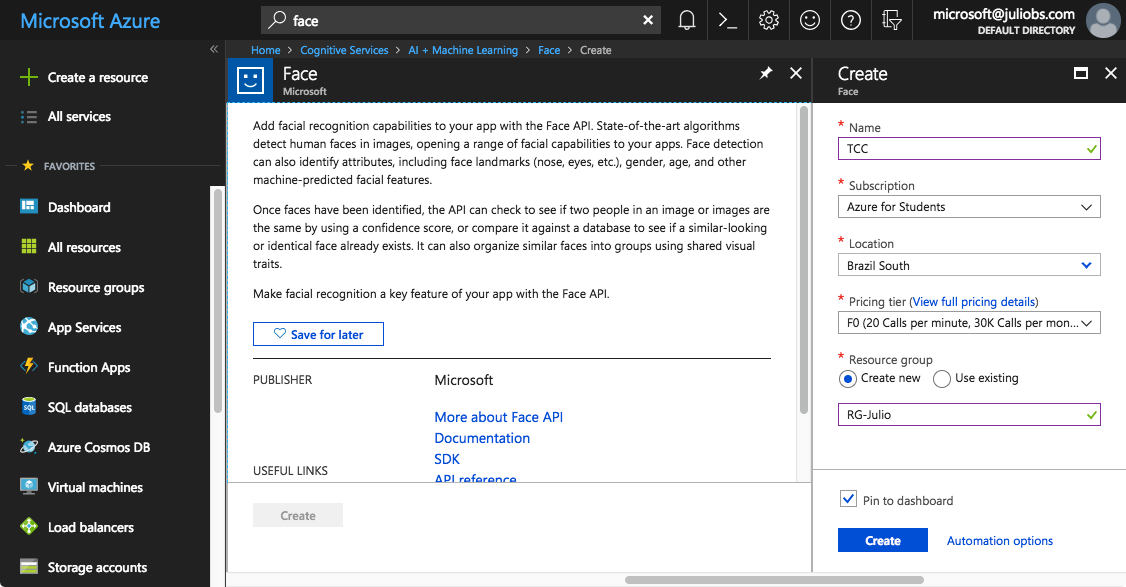
\includegraphics[width=0.95\linewidth]{imagens/azure_cria_face_api.png}
\end{figure}

\begin{figure}[htbp]
    \centering
    \caption{Teste da Microsoft Face API}
    \label{fig:face_api_test}
    \begin{subfigure}[t]{0.9\textwidth}
    \centering
    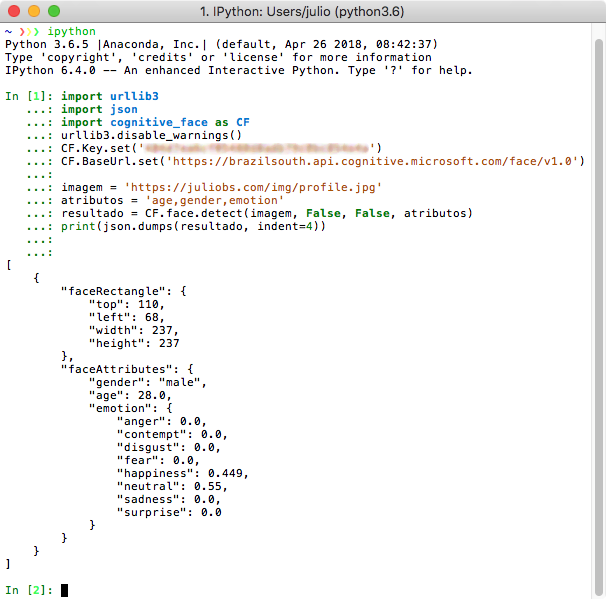
\includegraphics[width=0.8\linewidth]{imagens/msft_face_api_json.png}
    \caption{Python SDK para a Microsoft Face API} \label{fig:face_api_test:b}
    \end{subfigure}
    
    \vspace{\floatsep}
    \begin{subfigure}[t]{0.9\textwidth}
    \centering
    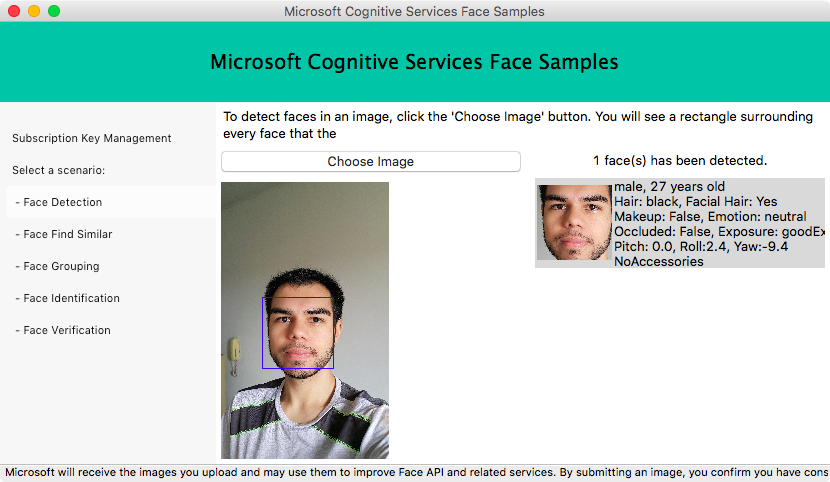
\includegraphics[width=0.8\linewidth]{imagens/msft_face_api_test.png}
    \caption{Aplicativo de exemplo} \label{fig:face_api_test:a}
    \end{subfigure}
\end{figure}